\documentclass[12pt]{article}

\usepackage[a4paper, left=2.5cm, right=2.5cm, top=2.5cm, bottom=2.5cm]{geometry}
\usepackage{times}

\usepackage[font=small, labelfont=bf]{caption}
\usepackage[subrefformat=parens]{subcaption}

\usepackage[indent=20pt]{parskip}
\usepackage{setspace}
%\onehalfspacing

\usepackage{graphics,graphicx}
\usepackage{svg}
\graphicspath{{../Figures/}}
\usepackage{mwe}

% Maths formatting
\usepackage{amsmath}

\usepackage{amsthm}
\newtheorem*{theorem}{Theorem}
\theoremstyle{definition}
\newtheorem*{definition}{Definition}
\newtheorem{condition}{Condition}

\usepackage[utf8]{inputenc}
\DeclareUnicodeCharacter{2212}{$-$} % Minus sign

% Bibliography
\usepackage[backend=biber, sorting=none, style=draft]{biblatex}
\addbibresource{thesis.bib}

% Number formatting
\usepackage[round-mode=figures,round-precision=3,round-pad=false,mode=text]{siunitx}

%\usepackage{multirow} % Multi-row cells in tables
%\usepackage{booktabs} % Nice table separators

% Clever references
\usepackage[hidelinks]{hyperref}
\usepackage[nameinlink,capitalise,noabbrev]{cleveref}
\crefname{condition}{Condition}{Conditions}

% Rename environments
\renewcommand{\listfigurename}{List of figures}
\renewcommand{\listtablename}{List of tables}

%\usepackage{float}

\title{\Huge \bfseries Quantum annealing\\for music arrangement}
\author{Lucas Kirby\\\normalsize Department of Physics, University of Durham\\\\\normalsize Supervised by\\\normalsize Prof Robert Potvliege \& Dr Omer Rathore}
\date{\normalsize 23 April 2025}

\begin{document}

\maketitle

\vfill

\addcontentsline{toc}{section}{Abstract}
\begin{abstract}              

Music arrangement is usually a complex and time-consuming process; this paper aims to provide an automatic method by which to arrange music via a quantum computing technique called quantum annealing. By splitting a score into a set of phrases, these phrases can form a quadratic unconstrained binary optimisation (QUBO), a function which the quantum computer aims to minimise by choosing the values of discrete variables. At the end of the optimisation process, the resulting chosen values describe the final arrangement, which can then be interpreted into sheet music. This method is tested on an excerpt of Beethoven's String Quartet No. 10 in E-flat major; in this case, the optimisation process is successful, and selects compatible phrases that produce a suitable arrangement.

\end{abstract}

\vfill

\begin{center}
    \includesvg{durham-university.svg}
\end{center}

\thispagestyle{empty}
\clearpage

\tableofcontents
\listoffigures
%\listoftables

\thispagestyle{empty}
\clearpage

\section{Introduction}

Music is often seen as a very human endeavour. For centuries, only skilled musicians could compose and perform such sequences of sound that would be considered art. Some would go one step further and adapt previously composed pieces for practical or artistic reasons, whether that be in terms of instrumentation, medium, or style, to create an \textit{arrangement}. One of the most famous examples of this is \textit{Pictures at an Exhibition}, a piano suite written by Modest Mussorgsky, but more commonly known for its orchestral arrangement by Maurice Ravel.
Traditionally, the arrangement of music is a complex process that requires a deep understanding of musical theory, structure, and style. Composers use their creativity and intuition to create a piece that is both musically interesting and emotionally engaging whilst still remaining faithful to the source material—a challenging and often time-consuming process. Perhaps it is unsurprising, then, that there has been interest in automating this process.

One of the earliest examples of this can be seen in the \textit{Musikalisches Würfelspiel} (``musical dice game'') system popular in the 18th century. The roll of dice would determine the order of pre-composed musical phrases, allowing for the creation of new music without the need for a composer. This system was engaged by the likes of Bach and Mozart, although fell out of fashion the following century.
The introduction of computers in the 20th century allowed for more sophisticated methods of music arrangement. Composers could now transpose and manipulate musical parts digitally, without the need to transcribe parts by hand. Moving into the 21st century, more advanced techniques such as genetic algorithms and neural networks have been used to arrange music, with varying degrees of success. However, these methods are limited by the complexity of the problem and the need for extensive training data.

The field of quantum computing has its foundations as early as the 1980s, with the suggestion that hardware following the laws of quantum mechanics could be faster and more powerful than its classical counterpart. Since then, two types of quantum computers have been developed: gate-based and annealing. Gate-based quantum computers, such as those developed by IBM  and Google , use quantum gates to manipulate qubits, the quantum equivalent of classical bits, and perform calculations. Quantum annealers, such as those developed by D-Wave Systems , use quantum fluctuations to find the global minimum of a given function. Each are suited to solving different classes of problems, with gate-based computers being more versatile and annealers being more efficient for certain optimisation problems. 

Quantum annealers are particularly well-suited to solving a class of problems known as NP-hard, defined in the field of computational complexity as an optimisation problem where the time taken to find a solution scales exponentially with the input size. A well-known example of an NP-hard problem is the travelling salesman problem, where the goal is to find the shortest route that visits a set of cities exactly once. This problem is difficult to solve because the number of possible routes grows rapidly with the number of cities. Quantum annealers have been shown to be effective at solving NP-hard problems, and have been used to find solutions to a variety of optimisation problems, such as protein folding , financial portfolios , and traffic flow .

The combination of quantum computing and music is a relatively new field, but one that has shown promise. Quantum computers have been used to write melodies , harmonies , create synthesisers , and even produce variations of original scores , using a mixture of gate-based and annealing methods. However, most of these efforts have been directed at music \textit{composition}, that is, the generation of entirely new sequences and sounds, rather than music \textit{arrangement}, an aspect with very practical use, due to the aforementioned significant skilled human effort this usually takes. Quantum computers have the potential to solve complex problems that are intractable for classical computers, and it is proposed that music arrangement is one such problem.

This paper will focus on a subset of music arrangement known as \textit{reduction}—taking a score written for a large number of parts and reducing it to a smaller number of parts, whilst still retaining the musicality and structure of the original. This is a common task in music production, where a piece written for a full orchestra may need to be arranged for a smaller ensemble, such as a string quartet. This forgoes the need to generate new music, as all notes in the arrangement are taken from the original score, and is more readily available to analyse as an optimisation problem.

In this study, the arrangement of a musical score is formulated as an NP-hard graph theory problem, by splitting the score into phrases with associated connections and weightings. This is then solved via a quantum annealer to produce a valid reduction according to imposed constraints. The final arrangement is visualised and evaluated, with suggestions for future work.

QNLP?

\section{Quantum annealing}

Before we consider quantum annealing, we must first discuss adiabatic quantum computing (AQC), from which it draws its main principle. AQC is a computing technique that works under the adiabatic theorem.

\begin{theorem}[Adiabatic theorem]
    A physical system remains in its instantaneous eigenstate if a given perturbation is acting on it slowly enough and if there is a gap between the eigenvalue and the rest of the Hamiltonian's spectrum. \cite{born_beweis_1928}
\end{theorem}

During a truly adiabatic process, there is no transfer of energy into or out of a system (??), so that system must remain in its energy eigenstate. This theorem can also be seen as a consequence of the energy-time uncertainty relation, which can be expressed as
\begin{equation}
    \Delta E\,T \ge \frac{\hbar}{2}
    \label{eq:energy-time}
\end{equation}
where here we define $\Delta E$ as the uncertainty in energy eigenstate and $T$ the time interval over which the system is evolved. As $T\to\infty$ we allow $\Delta E\to0$, meaning the exact energy eigenstate of the system can be known. A typical evolution of the Hamiltonian of the system can be expressed as
\begin{equation}
    H(t)=\left(1- \frac{t}{T}\right)H_0 + \frac{t}{T}H_p
    \label{eq:time-evolution}
\end{equation}
where we are evolving from an initial Hamiltonian $H_0$ to a final Hamiltonian $H_p$.
This technique is useful as it allows particular eigenstates (usually the ground state) of a very complicated Hamiltonian ($H_p$) to be found simply by evolving from a Hamiltonian whose eigenstate is easy to find and prepare ($H_0$). Importantly, this process is universal and deterministic---if the system starts in the ground state of $H_0$, then it is guaranteed to be in the ground state of $H_p$ after evolution.

However, since a truly adiabatic process takes infinitely many steps and therefore an infinite amount of time, this is not possible in practice. Instead, the adiabaticity condition of AQC can be relaxed to allow a shortening of the evolution time---this is quantum annealing\footnote{In metallurgical terms, annealing is the process of heating and cooling a material to alter its physical properties. Much like its metallurgical counterpart, quantum annealing allows a system to settle into a more useful final state.}. Over these shortened timescales ($T\sim\unit{\us}$), the process is now heuristic and the eigenstate after evolution is no longer guaranteed, but follows a probability distribution. The advantage of this method is that a particular evolution can be run many times, sampling the distribution of final states until an acceptable outcome is found.

The main use of quantum annealing is to solve combinatorial optimisation problems, which are problems that require the minimisation of a function over a discrete set of variables. If $H_p$ is prepared such that its ground state encodes the solution to the optimisation problem, then as long as the initial Hamiltonian is prepared in the ground state, the solution is likely to be given at the end of the annealing process. In the field of computational complexity, these problems belong to a class of complex problems called NP (nondeterministic polynomial-time). A full discussion of computational complexity is beyond the scope of this study, but in brief NP problems are difficult to solve via classical algorithms as the time to solution scales exponentially with problem size (hence nondeterministic). Problems like these have large solution spaces with many local minima, which cannot be solved quickly. A common example is the travelling salesman problem: a salesman must visit a set of cities exactly once and return home, whilst minimising the distance travelled [CHECK THIS]. As the number of cities increases, the number of possible routes the salesman could take grows exponentially, with a classical algorithm having to consider many more possible options. It is these sorts of optimisation problems that quantum annealers excel at solving.

In order to encode a problem, problem Hamiltonians ($H_p$) take the form of an Ising spin glass, a random arrangement of magnetic dipole moments (discrete variables) that can be in one of two states, typically spin-up ($+1$) or spin-down ($-1$) [CHECK THIS]. A spin glass with a vector $s$ of $N$ spins takes the form
\begin{equation}
    H(s) = \sum_{i<j}^{N}J_{ij}s_i s_j + \sum_{i=1}^{N}h_i s_i
    \label{eq:ising}
\end{equation}
where $J_{ij}$ are the coupling strengths between spins, and $h_i$ are the field strengths of individual spins. The quantum equivalent can be expressed as
\begin{equation}
    H_p = H(\sigma^z)
\end{equation}
where we have replaced the spins with Pauli matrices. This is the Ising model, with the discrete variables now \emph{qubits}---binary variables like their classical counterparts, but existing in a superposition of the two states until measurement. The corresponding ground state is prepared with the Hamiltonian
\begin{equation}
    H_0 = h_0\sum_{i=1}^{N}\sigma_i^x
\end{equation}
which is an equal superposition of all possible states in the eigenbasis of $H_p$ [CHECK THIS].

Another way of expressing problems is via the QUBO (quadratic unconstrained binary optimisation) model. A QUBO model takes the form of a function $f(x)$ to be minimised, and takes the form
\begin{equation}
    f(x)=\sum_{i<j}Q_{i,j}x_ix_j + \sum_iQ_{i,i}x_i
    \label{eq:qubo}
\end{equation}
where $x\in[0,1]$ is a new vector of binary variables, and $Q$ is an $N\times N$ upper-diagonal matrix of real weights. The off-diagonal $Q_{i,j}$ terms are known as quadratic coefficients, and diagonal $Q_{i,i}$ terms as linear coefficients. These two models are mathematically equivalent, and each can be transformed to the other via a change of variable
\begin{equation}
    s_i = 2x_i - 1 \,.
    \label{eq:qubo-ising}
\end{equation}
Whilst there are merits for each model, this study exclusively uses QUBO models to express optimisation problems.

\subsection{Quantum hardware}

% Should be near reference
\begin{figure}[b]
    \centering
    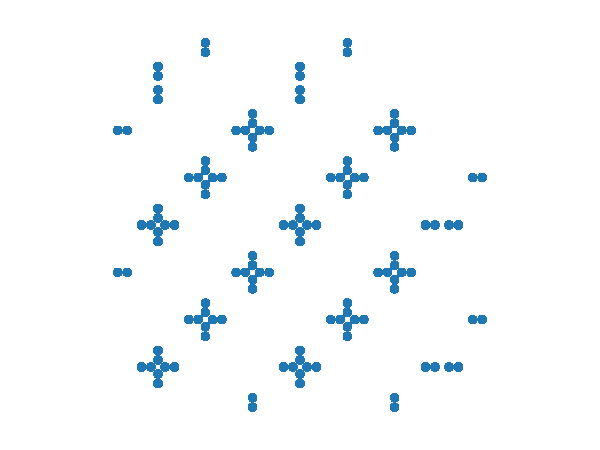
\includegraphics[width=0.5\linewidth]{../Figures/pegasus.pdf}
    \caption[A graph of \num{144} qubits in a D-Wave QPU.]{A graph of \num{144} qubits in a D-Wave QPU, using their Pegasus topology. Qubits are represented by vertices, and couplers by edges.}
    \label{fig:pegasus}
\end{figure}

Once a problem has been expressed with an Ising or QUBO model, it is sent to a quantum processing unit (QPU) to be solved. These units takes the form of a physical Ising spin glass, a lattice of physical qubits connected via couplers. The qubit biases and coupling values are influenced by electromagnetic fields, allowing the mapping of models to physical qubits, with linear terms as qubits and quadratic terms as couplers between them. This mapping process is known as \emph{minor embedding}, and is often handled by a classical computer `on the fly' each time a problem is submitted, introducing a slight computational overhead to running a problem. Fixed embeddings can be specified, but these require \textit{a priori} knowledge of the specific QPU architecture. Once embedded, the system can be prepared in its initial ground state, and allowed to evolve to its final state to obtain the solution.

Often, the topology of a QPU doesn't allow an exact one-to-one mapping of a problem to physical qubits. It may be the case that the problem requires a variable to have a higher degree (number of connections) than the number of couplers physically allowed by the QPU. The solution to this is the introduction of chains---connected physical qubits chained together, acting like a single discrete variable, which enables the necessary mapping. The chain strength determines how strongly the chain is coupled, enforcing that all qubits within the chain to have the same value in order for it to remain discrete. Chain strength is an important parameter that can affect the quality of solutions, and can be tuned. If it is too weak, a final state may include chain breaks: chains where the interconnected qubits differ in value. Conflicts like these can be solved via different approaches, a common one being majority vote, which sets the value of the corresponding discrete variable to the modal value of the chain. However, since this operation is done by a classical computer after the annealing process, the switch may result in an undesirable, sub-optimal solution, and so chain breaks are often best avoided. Alternatively, if the chain strength is too strong, it can overpower the other terms in the problem model, resulting in poor optimisation.

QPU annealers (also known as solvers) have many other parameters that can be tuned, influencing exactly how the annealing process is carried out and significantly affecting the quality of solutions [CITE SOLVER WEBSITE]. Aside from chain strength, others that this study considers are anneal time per sample and number of reads. Both these parameters affect the total QPU access time, and so finding a balance between them is key to minimising the time to solution.

As mentioned previously, the time interval for each sample (evolution) is short in order to relax the adiabatic condition. For simple problems this is sufficient to return optimal solutions with a high likelihood, however, as the problem size increases this may no longer be the case. For a problem with $N$ qubits there are $2^N$ energy levels, with the relative size of spectral gaps (differences between energy levels) decreasing with $N$ [ASK ABOUT THIS]. As seen in \cref{eq:energy-time}, smaller spectral gaps ($\Delta E$) require longer anneal times ($T$) to prevent excitation to higher energy states, such that the uncertainty in energy eigenstate is not large enough to eclipse this gap. (minimum energy gap?)

A benefit of shortened anneal times is that the system can be evolved and measured (sampled) many times, increasing the likelihood that a lower-energy solution from the distribution will be found. An evolution sampled many times creates a distribution in solution energy: for a simple QUBO model with a sparse matrix $Q$, this distribution may be biased towards lower energies therefore needing fewer samples; for a complicated matrix with many entries, the sampled distribution tends towards a Gaussian [RANDOM MATRIX LIT], with many more reads necessary to be likely to sample from the tail end. The density of a problem matrix can be found from the problem graph as:
\begin{equation}
    \rho=\frac{V+E}{V^2}
\end{equation}
where $V$ is the number of vertices and $E$ the number of edges, with $\rho=1$ indicating a fully-connected problem, the worst-case scenario.

% D-Wave
Many companies provide both personal and commercial access to gate-based quantum computers, however, few develop the hardware necessary for quantum annealing. D-Wave Systems was the first to realise a true quantum annealer, and have since developed and released their technology to the wider scientific community. All problems in this study were submitted to D-Wave's Advantage System 4.1 solver, which boasts a topology of over qubits each with a degree of. held at cryogenic temperatures and low-magnetic field environments to prevent unwanted fluctuations.

D-Wave Systems operates the first and only quantum annealer for commercial access, introduced in 2011 . All problems in this paper are run on the D-Wave Advantage quantum system, which uses their Pegasus architecture, an example of which can be seen in \cref{fig:pegasus}. A full Advantage QPU contains over \num{5000} qubits, each with a maximum degree of \num{15}.
Interaction with the D-Wave QPUs is handled through their Leap quantum cloud service, which is used to submit problems to solvers. D-Wave provides an open-source software development package (SDK) of Python tools which allows users to translate problems into binary optimisation and create problem models for the QPU to solve.

Quantum annealing has already been applied to a widge array of optimisation problems, ranging from financial portfolios, protein folding, and traffic flow. This study explores a creative novel application of this technique, music arrangement.

!!!Nick Chansellor paper, why quantum annealing?

\section{Music arrangement}
\label{sec:arrangement}

Music arrangement refers to the art of rewriting a musical score in a new setting, style, or structure, whilst still maintaining the essence of the original. A classical example of this is Mussorgsky's \emph{Pictures at an Exhibition}, which is well known for its orchestral arrangement by Ravel but was originally a piano solo. A more contemporary example would be ???'s rendition of \emph{The Star-Spangled Banner} at the ??? Super Bowl, which caused much controversy due to its laid-back style during a time of conflict in Cuba? The rearrangement of a piece can have a great effect on how the listener interprets it, and doing this effectively is still a pertinent issue many musicians face.

Traditionally, it's a time-consuming blah blah blah. However, in this study we aim to formulate music arrangement as an optimisation problem, which can be solved like any other via quantum annealing. It has been shown that music arrangement can be reduced to an NP-hard problem \cite{moses_computational_2016}, by considering the special case of music \emph{reduction}. Reduction is a form of arrangement whereby the number of instrument parts only gets smaller, and we define here subject to the following conditions:

\begin{condition}[Uncreative]
    All music in the arrangement must come from the original, in the same order.
    \label{con:uncreative}
\end{condition}
\begin{condition}[Non-degenerate]
    Music played in one arrangement part cannot be played in another.
    \label{con:non-degenerate}
\end{condition}
\begin{condition}[Monophonic]
    Each part in the arrangement can only contain music from a single part in the original at any time.
    \label{con:monophonic}
\end{condition}

Holistically, reduction aims to fit as much original music into the parts of the arrangement, whilst still being playable. Notably, these constraints forgo the need to compose new music, a very subjective endeavour that is not handled well by optimisation.

The beginning of any arrangement process is an original musical score. There exist a myriad of musical styles, genres, instruments, and notations, each as expressive and meaningful as the next. To maintain a manageable scope, this study focuses on European Classical-era (?) small ensemble and orchestral music, written in standard Western notation.

!!!mention somewhere score taxonomy (instruments, parts, polyphony, etc.)

% Theory, anyone could apply these steps. Then talk about practicalities in results (or in code appendix)
\section{Proposed framework}

Previous approaches to the automatic arrangement of music have relied on classical methods such as neural networks  or recursive classical algorithms in order to produce arrangements that are musically sound. However, these methods are limited by the complexity of the problem and the need for extensive training data. In this study, a new approach to the automatic arrangement of music is proposed by applying quantum annealing.

: given a set of musical phrases, each phrase can be assigned a binary variable and formulated into a Boolean satisfiability (SAT) problem, with variables assigned to clauses according to their compatibility. A valid solution would be an assignment of values such that the Boolean expression is satisfied, corresponding to the phrases included in the final arrangement . Phrases are chosen as the smallest unit of music instead of notes to best preserve important melodic lines and harmonies, which may sound dissonant or confusing if split up.

It has been shown that the arrangement of music can be formulated as a combinatorial optimisation problem \cite{moses_computational_2016}
We propose a new framework for the arrangement of music via quantum annealing, which has not been studied before at time writing. A toy example of the proposed method can be seen in \cref{fig:toy}.

\subsection{Score preprocessing}

The beginning of any arrangement process is an original musical score. However, before reduction can begin, the score must undergo preprocessing to ensure the produced arrangement will fulfil the conditions outlined in \cref{sec:arrangement}. In particular, \cref{con:monophonic} demands that all phrases must be strictly monophonic. Some instruments (e.g.\ strings) are capable of playing multiple notes at a time, whereas others (e.g.\ woodwind) physically cannot. Additionally, composers will often write several voice parts for orchestral sections, which can be played by individuals within the section simultaneosly. Both the cases of chords and voices break this condition, and so without knowing how phrases will be assigned, all music must therefore be reduced to monophony to ensure universal playability. We remove all but a single note from chords and multi-part voicings within the score before moving onto the next stage.

% Embedded metadata within the score allows it to be broken down into its constituent parts, bars, and notes, as well as containing information about the instrumentation and structure. Each note is represented by a vector of features, such as pitch and duration, as well as its position within the wider piece, which can be measured as an offset (the number of beats from the start of the score). 

\subsection{Phrase identification}

First, the music needs to be quantised. This could very easily be done by using predefined elements such as bars or notes, but these units on their own lack any intrinsic musical meaning. Similar to how a sentence might be split up into lexical phrases, instead of individial words or syllables, a line of music can be segmented into musical phrases, each representing a contained melodic or rhythmic idea. By preserving these important melodic lines and harmonies, we maintain the essence and familiarity of the original score, which is the core principle of arrangement as outlined in \cref{sec:arrangement}.

The approach taken in this study is the local boundary detection model (LBDM) \cite{cambouropoulos_lbdm_2011}, which aims to identify the boundaries between phrases by calculating the degree of change between successive notes; larger differences between notes would show an increased likelihood of a boundary, exploiting the fact that the starts and ends of phrases are usually characterised by a high degree of variation [CITE?]. The strength of a boundary on a particular note is calculated over two of its parameters: pitch, and inter-onset interval (IOI), the time until the next note. This is chosen over note duration as it is often more noticeable to the listener [CITE] (pithy quote about hearing the gaps between notes?). The boundary strength $S$ for a particular parameter $x$ at note $i$ is given by
\begin{equation}
    S_{x,i}=x_i\cdot (r_{i-1, i} + r_{i, i+1})
    \label{eq:boundary-strength}
\end{equation}
where $r_{i, i+1}$ is the degree of change of a parameter between notes $i$ and $i+1$, given by
\begin{equation}
    r_{i, i+1}=\frac{|x_{i}-x_{i+1}|}{x_{i}+x_{i+1}} \,.
    \label{eq:degree-change}
\end{equation}
In this way, a note with a high boundary strength would signal the start of a new musical phrase. The set of strengths for each parameter is normalised to the range $[0,1]$ (CHECK NOTATION) via
\begin{equation}
    S_{x,i}'=\frac{S_{x.i}-\min(S_x)}{\max(S_x)-\min(S_x)}
    \label{eq:normalisation}
\end{equation}
to ensure the analysis remains generalised across all pieces.
Finally, to find the total boundary strength, the strengths of each parameter are summed with a weighting, using weights derived by trial-and-error ($1/3$ for pitch and $2/3$ for IOI). The balance between these two parameters is a matter of taste and can be changed based on the perceived accuracy of the identified boundaries. If a note's total boundary strength surpasses a specified threshold, it is considered a boundary and signals the start of a new phrase. Boundaries are always taken at the beginning and end of a score.

This model is run on each instrument part in a score; once a list of boundaries is created, the phrases can be defined by taking a boundary and the one following as the start and end points. Each phrase is labelled according to the part it belongs to and its phrase index within that part, allowing the phrases to be easily referenced and reconstructed into a new score once the optimisation is complete. An example of the output of the LBDM can be seen in \cref{fig:toy-phrases}.

\subsection{Problem formulation}

How can the arrangement of these phrases, in fulfilment of the constraints outlined previously, be expressed as an optimisation problem that can be solved via quantum annealing? There are many pre-existing NP problems that can be solved in this way, including Boolean satisfiability and set theory \cite{lucas_ising_2014}. Here we show that the music arrangement problem can be reduced to a graph theory problem known as \emph{proper vertex colouring}.

A graph $G$ can be defined as $G=(V,E)$, where $V$ is a set of vertices (or nodes) and $E$ is a set of edges that defines relationships between the vertices. Vertices are considered `adjacent' or `connected' if they have an edge between them. These constructions (?) are useful to model pairwise relations between objects, and there exist a number of graph optimisation problems, each with a variety of applications.\footnote{The travelling salesman problem is often represented as a graph theory problem, with vertices representing cities and edges the routes between them.} This study uses a problem in the category of graph colouring known as proper vertex colouring.

\begin{definition}[Proper vertex colouring]
    The assignment of colours to the vertices of a graph such that no two adjacent vertices share the same colour.
\end{definition}

In this case, each phrase is represented by a vertex, with edges connecting vertices that overlap (i.e.\ played different parts at the same time). The assignment of `colours' to these vertices then represents the part in the arrangement that plays the phrase. An example of a graph constructed in this way can be seen in \cref{fig:toy-graph}. This can be seen to fulfil the conditions outlined previously: \cref{con:uncreative} is met by only considering phrases identified from the original score; \cref{con:non-degenerate} is met by only allowing each vertex at most one colour, preventing a phrase being played twice simultaneously; \cref{con:monophonic} is met by adjacent colours constraint, meaning a single part cannot play two overlapping phrases simultaneously. 

If we define $x_{v,i}$ to be a binary variable such that
\begin{equation}
    x_{v,i} =
    \begin{cases}
        1 & \text{if vertex $v$ is colour $i$} \\
        0 & \text{otherwise}
    \end{cases}
    \,,
\end{equation}
for a set of $n$ colours then the QUBO model for proper vertex colouring can be expressed as
\begin{equation}
    f(x)=A\sum_{v \in V}\left(s_v-\sum_{i=1}^{n} x_{v,i}\right)^2+B\sum_{(u,v) \in E}\sum_{i=1}^n x_{u,i}x_{v,i}
    \label{eq:colouring}
\end{equation}
where $A,B$ are the Lagrange parameters, and we have introduced the slack variables $s_v\in\{0,1\}$ (CHECK NOTATION).\footnote{This reduces to the maximum independent set problem when $n=1$.} The first term implements the single-colour constraint (or vertex constraint) by increasing the energy by $A$ each time a vertex is coloured more than once. The nature of a reduction implies that not all phrases will be played, so the inclusion of the slack variables (specifically when $s_x=0$) allows a vertex not to be coloured at all. Similarly, the second term implements the colour-adjacency constraint (or edge constraint) by increasing the energy by $B$ for each pair of identically-coloured vertices connected by an edge. When this function is minimised (strictly zero, in this case), all the conditions are met for a valid arrangement. The $x_{v,i}$ can then be read off from the solution and cross-referenced with their corresponding phrases to give the final score, an example of which can be seen in \cref{fig:toy-arrangement}.

\begin{figure}
    \begin{subfigure}{0.5\textwidth}
        \includegraphics[width=\linewidth]{example-image-a}
        \caption{}
        \label{fig:toy-phrases}
    \end{subfigure}\hfill
    \begin{subfigure}{0.5\textwidth}
        \includegraphics[width=\linewidth]{example-image-b}
        \caption{}
        \label{fig:toy-graph}
    \end{subfigure}
    \begin{subfigure}{0.5\textwidth}
        \includegraphics[width=\linewidth]{example-image-b}
        \caption{}
        \label{fig:toy-solution}
    \end{subfigure}\hfill
    \begin{subfigure}{0.5\textwidth}
        \includegraphics[width=\linewidth]{example-image-a}
        \caption{}
        \label{fig:toy-arrangement}
    \end{subfigure}

    \caption[A toy example demonstrating the proposed framework.]{A toy example demonstrating the proposed framework. \subref{fig:toy-phrases} An example score of three parts, with phrases identified by the LBDM coloured. \subref{fig:toy-graph} A graph of the score, with the colour of each node corresponding to its phrase, and edges connecting overlapping phrases. \subref{fig:toy-solution} One possible solution of proper vertex colouring, with $n=2$. \subref{fig:toy-arrangement} The score representation of the final arrangement.}
    \label{fig:toy}
\end{figure}

\subsection{Musical entropy}

A valid arrangement of phrases does not good music make. To ensure the produced arrangement is as musically interesting as possible, each vertex of the graph can be weighted to introduce a bias according to its phrase's `musicality'. The idea of a musical `utility' has been used before with classical algorithms \cite{huang_towards_2012} and to assess playability rules [PIANO REDUCTION CITATION]. Here we quantify this by calculating the \emph{musical entropy} of a phrase \cite{li_entropy_2019}.

Entropy can be seen as how much information a variable contains; in this context, a phrase with a higher entropy would indicate a higher level of variation and complexity, increasing the likelihood of it being more `musical'. Maximisation of phrase entropy would then result in the creation of richer arrangements. For a discrete random variable $X$ with a probability distribution $P(X)$, the Shannon entropy is defined as
\begin{equation}
    H(X):=-\sum_i P(x_i)\log_2 P(x_i)
    \label{eq:entropy}
\end{equation}
where each $x_i$ is a possible value of $X$ and ${\sum_i P(x_i)=1}$. In this context, the random variable is a musical note, considering its possible values in terms of both pitch and duration.

Pitch entropy is calculated by considering the distribution of pitches in a phrase. The probabilities of each pitch $x_i$ can be found by
\begin{equation}
    P(x_i)=\frac{n_i}{N}
    \label{eq:prob-dist}
\end{equation}
where $n_i$ is the number of times pitch $x_i$ appears in the phrase and $N$ is the total number of notes in the phrase. A phrase with a greater variety of pitches (and thus greater entropy) will likely be more `interesting' and so should have a higher bias to be included in the final arrangement.
Rhythm entropy is calculated in a similar manner, but considering the duration of the note instead. This is also calculated using \cref{eq:prob-dist}, but instead considering $x_i$ as possible duration values.
The total entropy of a phrase is then the sum of the pitch and rhythm entropies.

We can modify \cref{eq:qubo} to include vertex weights by adding an objective term that looks like
\begin{equation}
    f_C(x)=-C\sum_{v\in V}\sum_{i=1}^n W_v x_{v,i}
\end{equation}
where $W$ is a vector holding the weights for each vertex, and $C$ is the associated Lagrange parameter. Objective terms are negative to ensure than the minimisation of this function results in the maximisation of the objective (the sum of the total weights).

Weights can also be added to edges, to bias the selection of pairs of vertexes. Here we assign edge weights as the absolute difference between the weights of the vertices it connects, adding a tendency to colour connected vertices that have very different weights. Musically, this means simultaneous phrases are more likely to be picked if their musical entropies differ; complex, strongly varying, high-entropy phrases may sound noisy and confusing if played together, so this choice allows each high-entropy phrase to be accompanied by a simpler, low-entropy one. The associated objective term modification to \cref{eq:qubo} looks like
\begin{equation}
    f_D(x)=-D\sum_{(u,v)\in E}W_{uv}\sum_{i=1}^n\sum{i<j}^n x_{u,i}x_{v,j}
\end{equation}
where $W$ is now a matrix holding the weights for each edge, and $D$ is the Lagrange parameter.

Finally, we introduce a bias towards the assignment of vertices to specific colours, based on the instrument the colour represents. It has been shown that instrument parts within a score can be categorised into distinct `arrangement elements', or roles, which reflect their musical function within the piece \cite{owsinski_mixing_2017}. Here we consider only three: lead, often including melodic/countermelodic lines; rhythm, providing harmony; and foundation, the fundamental bass line. Rudimentarily, we can classify phrases into these three categories by their entropy. Melodic lines often vary more, have higher entropy, and therefore should be classed as lead, whereas lower-entropy phrases should tend towards rhythm or bass. By defining threshold entropy values for each category, phrases can be given a bias towards instruments that have been assigned that category. For example, a flute part assigned a lead in the arrangement should contain more high-entropy phrases than a cello part assigned as foundation. The corresponding objective term takes the form
\begin{equation}
    f_E(x) = -E\sum_{v\in V}\sum_{i=1}^n \theta(W_v - W_{\text{th},i})x_{v,i}
\end{equation}
where $W_{\text{th},i}$ is the threshold value for the category of instrument $i$, $\theta$ is the Heaviside step function, and $E$ is the Lagrange parameter.

Together, the final QUBO model is
\begin{align}
    f(x)&=f_{A,B}+f_C+f_D+f_E \notag\\
    &=A\sum_{v \in V}\left(s_v-\sum_{i=1}^{n} x_{v,i}\right)^2+B\sum_{(u,v) \in E}\sum_{i=1}^n x_{u,i}x_{v,i} \notag\\
    &-C\sum_{v \in V}\sum_{i=1}^n W_vx_{v,i}-D\sum_{(u,v)\in E}W_{uv}\sum_{i=1}^n\sum_{i<j}^n x_{u,i}x_{v,j}-E\sum_{v \in V}\sum_{i=1}^n\theta(W_v-W_{\text{th},i})x_{v,i}
    \label{eq:problem-qubo}
\end{align}
which requires $N(n+1)$ variables, where $N$ is the total number of phrases.

\subsection{Lagrange parameter analysis}

To ensure that the minimisation of \cref{eq:problem-qubo} does indeed fulfil the constraints necessary for a valid arrangement as outlined before, the Lagrange parameters must be tuned. It is possible for this to be done \textit{a priori} [CITE], however, with five parameters, a full parametric analysis would be complicated, so this study focuses on an empirical approach.

Nonetheless, a quick algebraic calculation can help reduce the problem. The model given by \cref{eq:problem-qubo} contains two constraints, each which aims to fulfil a different condition. The vertex constraint (labelled with $A$) upholds \cref{con:non-degenerate}, the breaking of which would introduce phrases being duplicated across parts in the final arrangement. The edge constraint (labelled with $B$) upholds \cref{con:monophonic}, preventing phrases that overlap being played by the same part. The number of duplicates and overlaps needs to be strictly zero in order for a solution to be valid therefore these Lagranage parameters need to be large enough to facilitate this.

In a worst-case scenario, a vertex included in the solution would lower the energy maximally whilst breaking a constraint. To ensure that this results in an overall increase in energy, and is therefore less likely, we can derive the inequality
\begin{equation}
    A + B > C\max(W) + D\max(W) + E
\end{equation}
where $\max(W)$ denotes the largest entry of the weight matrix. To allow a similar analysis across problems with different weights, we set $C=D=1$ and introduce new parameters $X_m$ that scale with the maximum weight, such that $X = X_m\max(W)$, giving us the expression
\begin{equation}
    A_m + B_m > 2 + E_m \,.
    \label{eq:lagrange}
\end{equation}

In this study we set $E_m=1$ as bias towards part types is preferred but not essential. The values of $A_m$ and $B_m$ can then be found by performing parametric variation and measuring the number of broken constraints (duplicates and overlaps) in the lowest energy solutions. Parameter values should be just large enough to fulfil constraints, whilst not being too large as to overwhelm the other terms in the QUBO equation [CITE] and affect the quality of solutions.

\subsection{Solution interpretation}

Once the problem has been submitted to a quantum annealer and a sample set returned, we can finally construct the arrangement. Of the distribution of samples, the lowest-energy valid (i.e.\ no duplicates or overlaps) sample is picked to be the solution. The binary variables assigning vertices to colours can be read off and interpreted as phrases and instruments, respectively, allowing the music of the original score to be transformed into the final arrangement.

This is the point where music post-processing can be applied. In this study, phrases are shifted up or down octaves depending on the pitch range of the target instrument, to ensure playability whilst minimally affecting the essence of the original.

\section{Results}

The outlined framework was applied to two scores: Quartet No.\ 1 in B-flat major, Op.\ 1, by Joseph Haydn, and Symphony No.\ 5 in C minor, Op.\ 67, I.\ Allegro con brio, by Ludwig van Beethoven. Haydn Op.\ 1 is of the Baroque style, consisting of 63 bars with four instrument parts that play consistently throughout the piece, structured into short, well-defined phrases. This score was chosen as it was expected that the LBDM would be reasonably successful in discretising the piece, and that its short length and smaller instrumentation would result in a manageable number of variables to be embedded in the QPU. Beethoven Op.\ 67 is of the Romantic style and was shortened to the first 21 bars, with 12 instrument parts that are introduced at different times in the piece. This score was chosen for limit-testing purposes, as its larger instrumentation greatly increases the connectivity of the problem. Notably, the piece is also very well-known meaning the constructed arrangements would be more familiar.
Original scores, and their reduction counterparts, can be found in \cref{app:examples}.

The results of the LBDM can be seen in \cref{fig:phrase-extraction}. Notes with boundary strengths above the chosen threshold were chosen to be boundaries, defining the phrases that would become the vertices of the problem graph. The entropy of each phrase was calculated using \cref{eq:entropy}, to be used as the corresponding vertex weight, and the QUBO model was then calculated using \cref{eq:problem-qubo}, which could then be sent to the QPU to be solved.

Tuning of the Lagrange parameters can be seen in \cref{fig:lagrange}. The parameters used for subsequent models were $A=6$ and $B=6$, which can be seen to fulfil \cref{eq:lagrange} as expected. Each constraint parameter guarantees an increase in energy roughly double the potential energy decrease for a broken constraint, a value which has been shown before (???) [CITE LIT].

An example of the distribution of a returned sample set can be seen in \cref{fig:histogram}. The most optimal solutions lie in the leftmost portion of the distribution, corresponding to the lowest energies. The Gaussian nature of this distribution changed very little throughout parameter configuration process, hinting at the possibility that the problem models were already complicated enough to resemble random matrices. How sparse is the problem graph? $(nodes + edges)/nodes^2$

Optimisation of both chain strength and anneal time per sample can be seen in 

Music can be represented by many digital formats, each with their own benefits---in this study we choose to use MusicXML [CITE], a variant of the well-establish XML (extensible markup language) format. This format focuses on the interactive representation of standard sheet music, describing musical notes, rests, and other symbols, as well as the structure of the music, such as the arrangement of notes into bars, parts, and scores. It is widely supported by music notation software, allowing translation of music to graphic (PDF, PNG) and audio (MIDI, MP3) formats, as well as Python libraries that provide extensive resources for manipulating, translating, and creating MusicXML files, allowing scores to be broken down and reconstructed as fit.\footnote{An overview of the code resources used in this study can be found in \cref{app:code}.} Although not as prevalent as other file formats, there exist a number of online libraries and databases of MusicXML files provided in the public domain.

\begin{figure}
    \begin{subfigure}{0.5\textwidth}
        \includegraphics[width=\linewidth]{example-image-a}
        \caption{}
    \end{subfigure}\hfill
    \begin{subfigure}{0.5\textwidth}
        \includegraphics[width=\linewidth]{example-image-b}
        \caption{}
    \end{subfigure}
    \caption{Phrase extraction as a result of the LBDM.}
    \label{fig:phrase-extraction}
\end{figure}

\begin{figure}
    \includegraphics[width=.5\textwidth]{example-image-a}
    \caption{Histogram example of a returned sample set.}
    \label{fig:histogram}
\end{figure}

\begin{figure}
    \begin{subfigure}{0.5\textwidth}
        \includegraphics[width=\linewidth]{example-image-a}
        \caption{}
    \end{subfigure}\hfill
    \begin{subfigure}{0.5\textwidth}
        \includegraphics[width=\linewidth]{example-image-b}
        \caption{}
    \end{subfigure}
    \caption{Tuning Lagrange parameters.}
    \label{fig:lagrange}
\end{figure}

\begin{figure}
    \begin{subfigure}{0.5\textwidth}
        \includesvg[width=\linewidth]{chain-strength.svg}
        \caption{}
    \end{subfigure}\hfill
    \begin{subfigure}{0.5\textwidth}
        \includegraphics[width=\linewidth]{example-image-b}
        \caption{}
    \end{subfigure}
    \caption{Chain strength and anneal time per sample.}
    \label{fig:solver-config}
\end{figure}

\begin{figure}
    \begin{subfigure}{0.5\textwidth}
        \includegraphics[width=\linewidth]{example-image-a}
        \caption{}
    \end{subfigure}\hfill
    \begin{subfigure}{0.5\textwidth}
        \includegraphics[width=\linewidth]{example-image-b}
        \caption{}
    \end{subfigure}
    \caption{Comparison with classical solvers varying number of reads.}
    \label{fig:reads}
\end{figure}

\begin{figure}
    \begin{subfigure}{0.5\textwidth}
        \includegraphics[width=\linewidth]{example-image-a}
        \caption{}
    \end{subfigure}\hfill
    \begin{subfigure}{0.5\textwidth}
        \includegraphics[width=\linewidth]{example-image-b}
        \caption{}
    \end{subfigure}
    \caption{Scaling with number of instruments.}
    \label{fig:energy-scaling}
\end{figure}

\begin{figure}
    \includegraphics[width=.5\textwidth]{example-image-a}
    \caption{Increase in variables with number of instruments (one for linear terms one for quadratic terms)}
    \label{fig:qubit-scaling}
\end{figure}

\begin{figure}
    \includegraphics[width=.5\textwidth]{example-image-a}
    \caption{Comparing time to solution with number of instruments}
    \label{fig:times}
\end{figure}

\begin{itemize}
    \item Lagrange parameter variations
    \item 2D surface plot?
    \item Compare to analytic derivation (reference for double value?)
\end{itemize}



Having tuned the Lagrange parameters and sampler configuration to give the lowest energy possible, we can compare the returned solutions to classical optimisation algorithms solving the same problem. D-Wave provides a selection of classical samplers that can return solutions to QUBO problems, two of which are used in this study. The steepest descent method blah blah. Simulated annealing, on the other hand, works very similarly to quantum annealing, but instead uses a "temperature" value to escape local minima. This method gives a more direct comparison.

Show energy against reads
Show total entropy against reads

\begin{enumerate}
    \item Score length
    \item Number of instruments
\end{enumerate}

Phrases identified using the LBDM are shown in Fig.\  , alongside their calculated entropies according to Eq.\ \ref{eq:entropy} and their overlaps, represented by edges. A threshold value of $0.4$ was used, resulting in a total of 33 identified phrases, with 70 total overlaps. The calculated boundary strengths for the Violin 1 part can be seen in Fig.\ \ref{eq:boundary-strength}, with the identified boundaries summarised in Tab.\ . Many of the nodes form cliques of three or four vertices, that is, each node of the subset is connected to every other node. This can be expected, as often musical phrases across instruments will occur simultaneously, especially in small ensemble music such as this. Notably, there are also two disjoint cliques, subsets that are independent from the main graph. These can be seen as distinct musical ideas that are separated by rests from the other phrases (for example, the first two measures of the piece). A non-negligible number of phrases are calculated to have zero entropy—these are phrases identified as only having one note, and thus no variety in pitch or rhythm ($P(x_i)=1$).

The QUBO was calculated using, with Lagrange parameters $A=11.5$ and $B=1$. The value of $A$ was chosen to be twice the maximum node weight (phrase entropy) such that the penalty of choosing a node that introduces an edge into the solution would likely outweigh any possible benefit of its weighting. After submission of the QUBO to the D-Wave QPU, a sample set of solutions was returned, which can be seen in Fig.\  . Many solutions had degenerate energies—the lowest energy was -26.821803 with a degeneracy of 34 and zero chain breaks. These solutions used slightly different combinations of phrases to make the maximal independent set; this degeneracy is likely due to the high number of cliques, which only allows one node of the subset to be picked, and phrases with zero entropy, which do not change the final energy when interchanged. One of the lowest energy solutions can be seen in Fig.\  , with the nodes selected by the QPU highlighted. In this solution, none of the nodes are connected by edges, providing a valid monophonic arrangement. The musical score of this solution is shown in Fig.\  .

!!!comparing time to solution
For QA only looking at annealing time, not QPU access time (which includes sampling, readout, programming time) as this is a limitation of the technology rather than the method

\section{Conclusions}

% Limitations

Although the technology has been improving for several years, at time of writing quantum annealers are still in the development stage. D-Wave's latest chip, the Advantage 4.1, boasts a topology of over \num{5000} vertices

QPU chip graph size -> affects length of scores/granularity of phrases/number of arrangement instruments
!!!is possible to partition graphs to reduce problem sizes (include citation) but is future work

Maximum problem time limit -> affects maximum time per anneal which could affect quality of results

Removing chords and voices from scores -> loss of information

!!!what is the main limiting factor?
Computers aren't big enough yet, but how big would they need to be? Look into new Zephyr topology

!!!future work
reverse annealing
change in anneal schedule, pause/quench
graph partitioning
a priori lagrange parameters (Nelder-Mead)
unbalanced penalisation vs slack penalisation (would reduce number of variables)


In the case of Beethoven's String Quartet No.\ 10, this method can be said to be successful in reducing the score to a single monophonic part. A sufficient number of phrases are identified to allow the key melodic lines to be picked out from each part, and the weighted MIS formulation results in a final arrangement that is not musically uninteresting. Here, only one solution was picked arbitrarily; if desired, each of the degenerate lowest energy solutions could be examined individually to isolate the one that is considered most ``musical'', safe in the knowledge that all of them are valid.

One advantage this method has over classical algorithms is that no training data is needed. Genetic and deep learning approaches require refinement of their models on large datasets, ``teaching'' what a valid arrangement looks like, which takes considerable time and resources. By using a QPU, these ``rules'' can effectively be encoded using constraints, such as the penalty term introduced into the QUBO; as long as these constraints are fulfilled, the QPU will always provide a feasible solution, without any knowledge of previous arrangements.

Another benefit is the solve time: for the problem graph shown in Fig.\  , the D-Wave QPU access time (the time taken to embed and solve the problem) is approximately 150 ms for 1000 reads. Compared to classical methods using a similar number of phrases, the quantum process is faster by at least one order of magnitude . For classical computers, the time taken to solve NP-hard problems increases exponentially with the problem size, so this speed advantage will only improve as the scores become more complex.

Future work would include testing this process on a wide range of pieces from different musical styles. Scores from different time periods (Baroque vs.\ Romantic, for example) have wildly different structures, and so the effectiveness of the LBDM could vary in identifying suitable musical phrases. The treatment of melodic lines between different ensembles, whether that be a string quartet or symphony orchestra, also varies, and the isolation of important melodic lines may become more difficult.

To that regard, the effect of LBDM parameters (pitch/IOI weighting, threshold) on phrase identification could be studied. Ideally, musical phrases should be fairly short and similar in length, to give the MIS algorithm the best chance in selecting the most interesting sections of the score. This would prevent important notes being hidden in long phrases with low entropy. Other boundary detection methods could also be tested, with their resulting identified phrases compared qualitatively.

Currently, no regard is taken to the exact instrumentation of the final arrangement. Different instruments have varying ranges of pitches that can physically be played; here, phrases have been chosen from across all the instrument parts (as seen in Fig.\  ), however, this does not mean that the final arrangement can be played by all the instruments as some notes may be unfeasible. Care needs to be taken to check the ambitus (pitch range) of chosen phrases and ensure that it falls within the desired instrument's range; if not, phrases can be transposed by octaves up or down without altering the melodies significantly.

The MIS formulation works well for reducing a score into a single polyphonic part, as the inclusion of a phrase within the final arrangement lends naturally to the binary variables used. However, a more useful application would be the ability to reduce a score to any fewer number of parts, whether that be multiple monophonic instruments (e.g.\ string quartet) or a polyphonic instrument (e.g.\ piano). To achieve this, the QUBO would need to be altered to allow some edges into the final subset. One suitable formulation would be a graph colouring problem: colouring the vertices of a graph $G$ with a set of $n$ colours such that no edge connects two vertices of the same colour. In this context, the number of colours would be the number of desired parts—after solving, each disjoint set of colours would become a monophonic part, the combination of which becomes the final reduction (in this way, the MIS problem can be seen as a colouring problem where $n=1$).

Although it can be argued that music cannot be objectively ``scored'', nonetheless, the quality of the produced arrangements needs to be judged in some way. One suggestion is that the ``goodness'' of music can only be measured via a Turing-like test, where human subjects are presented with a selection of both human- and computer-generated scores, and asked to categorise them . To this extent, a good measure of the arrangements produced by this method would be to compare them against popular arrangements of the same score composed by human professionals, via a series of blind trials. If the participants fail to identify the computer compositions from the human ones more often than random chance, then it can be said that the generated arrangements are of sufficiently good quality.

To conclude, this paper has shown the automatic reduction of music via quantum annealing. By formulating a score into a function to be minimised, the annealing process can identify parts of the original to become the final arrangement. An automatic process of this sort would be useful to a wide calibre of musicians, removing the time and skill barrier to produce such arrangements, whilst still retaining a sufficient level of quality, keeping music accessible to all. Just as science and business do already, it can be hoped that the arts take advantage of promising new technologies as well.

% References
\printbibliography[heading=bibintoc]

\clearpage
\appendix

\section{Code overview}
\label{app:code}

\section{Examples}
\label{app:examples}

\begin{figure}
    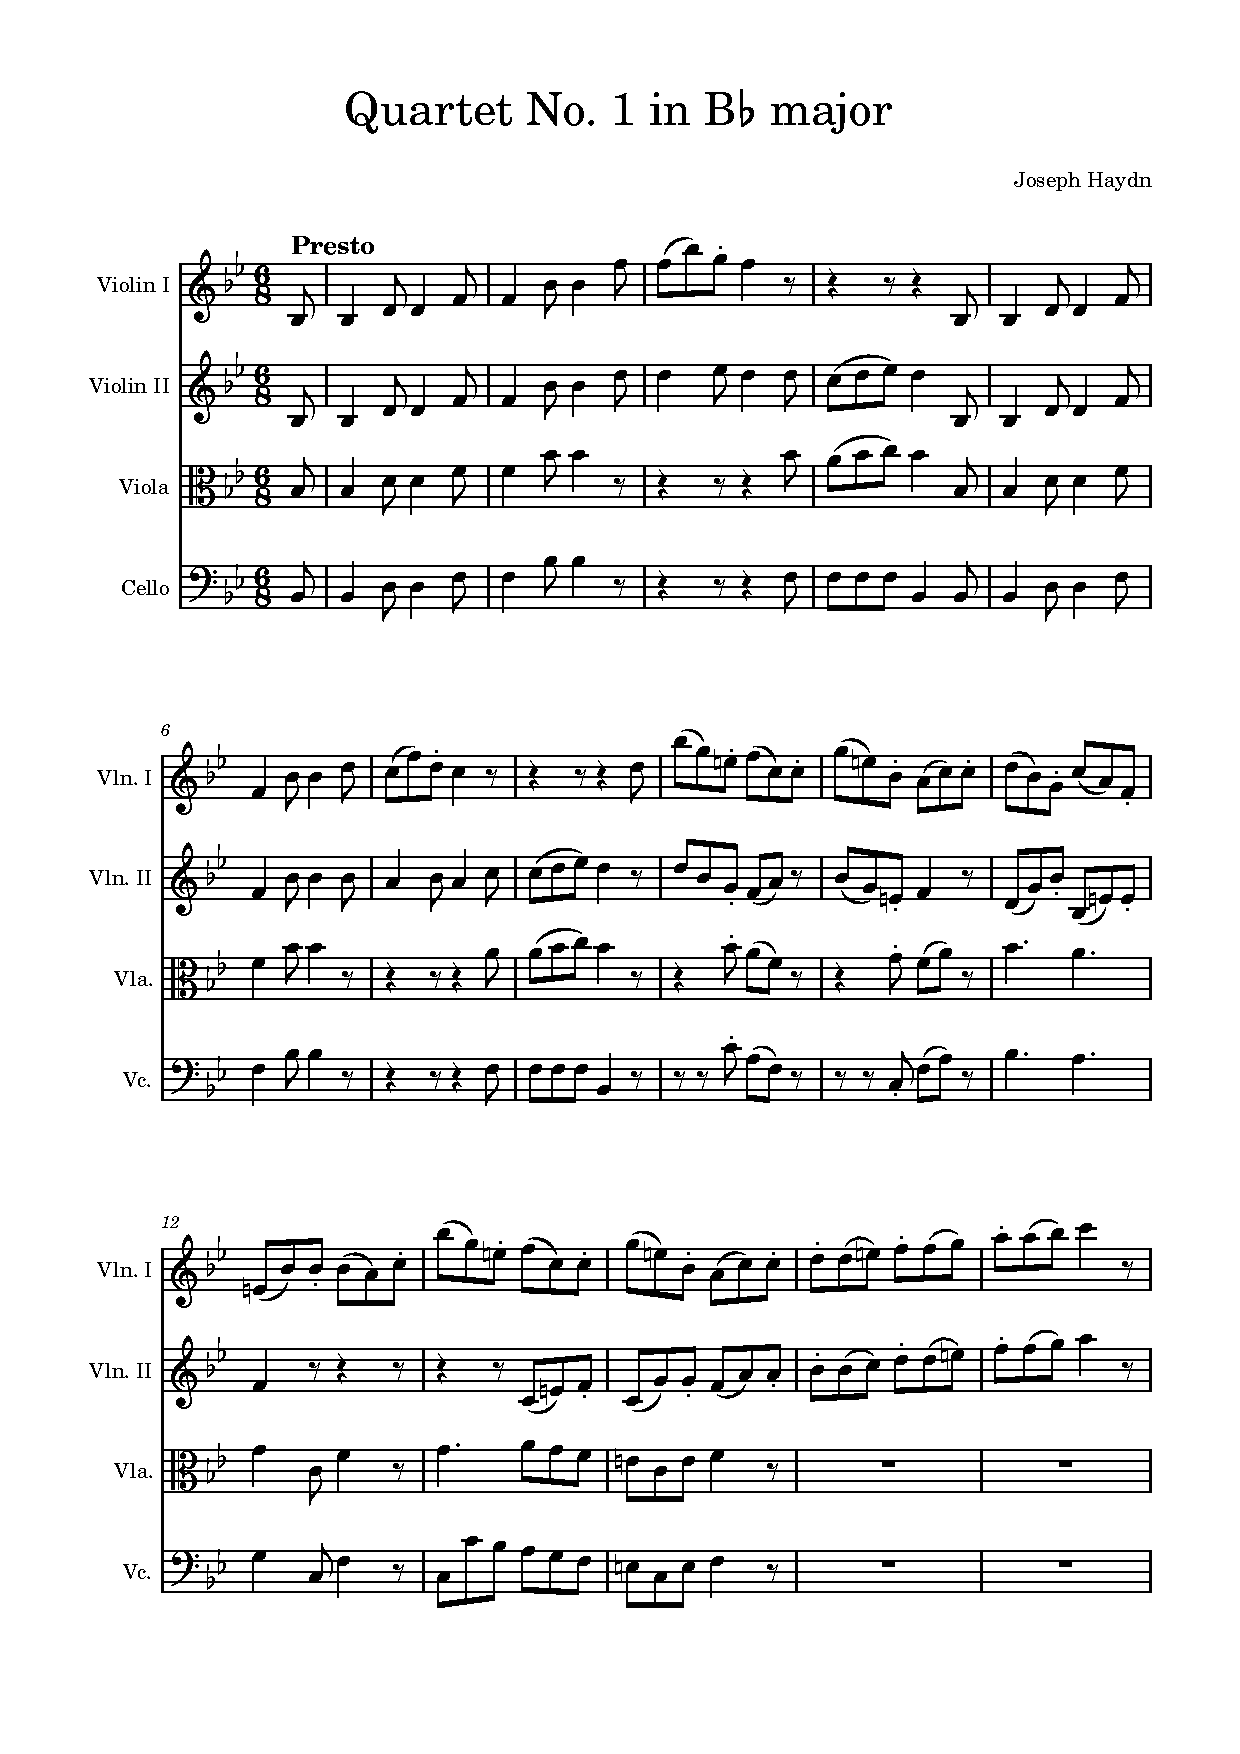
\includegraphics[width=\textwidth,page=1]{haydn-op1.pdf}
    \caption{Quartet No.\ 1 in B-flat major, Op.\ 1, by Joseph Haydn, bars 1--16.}
\end{figure}

\begin{figure}
    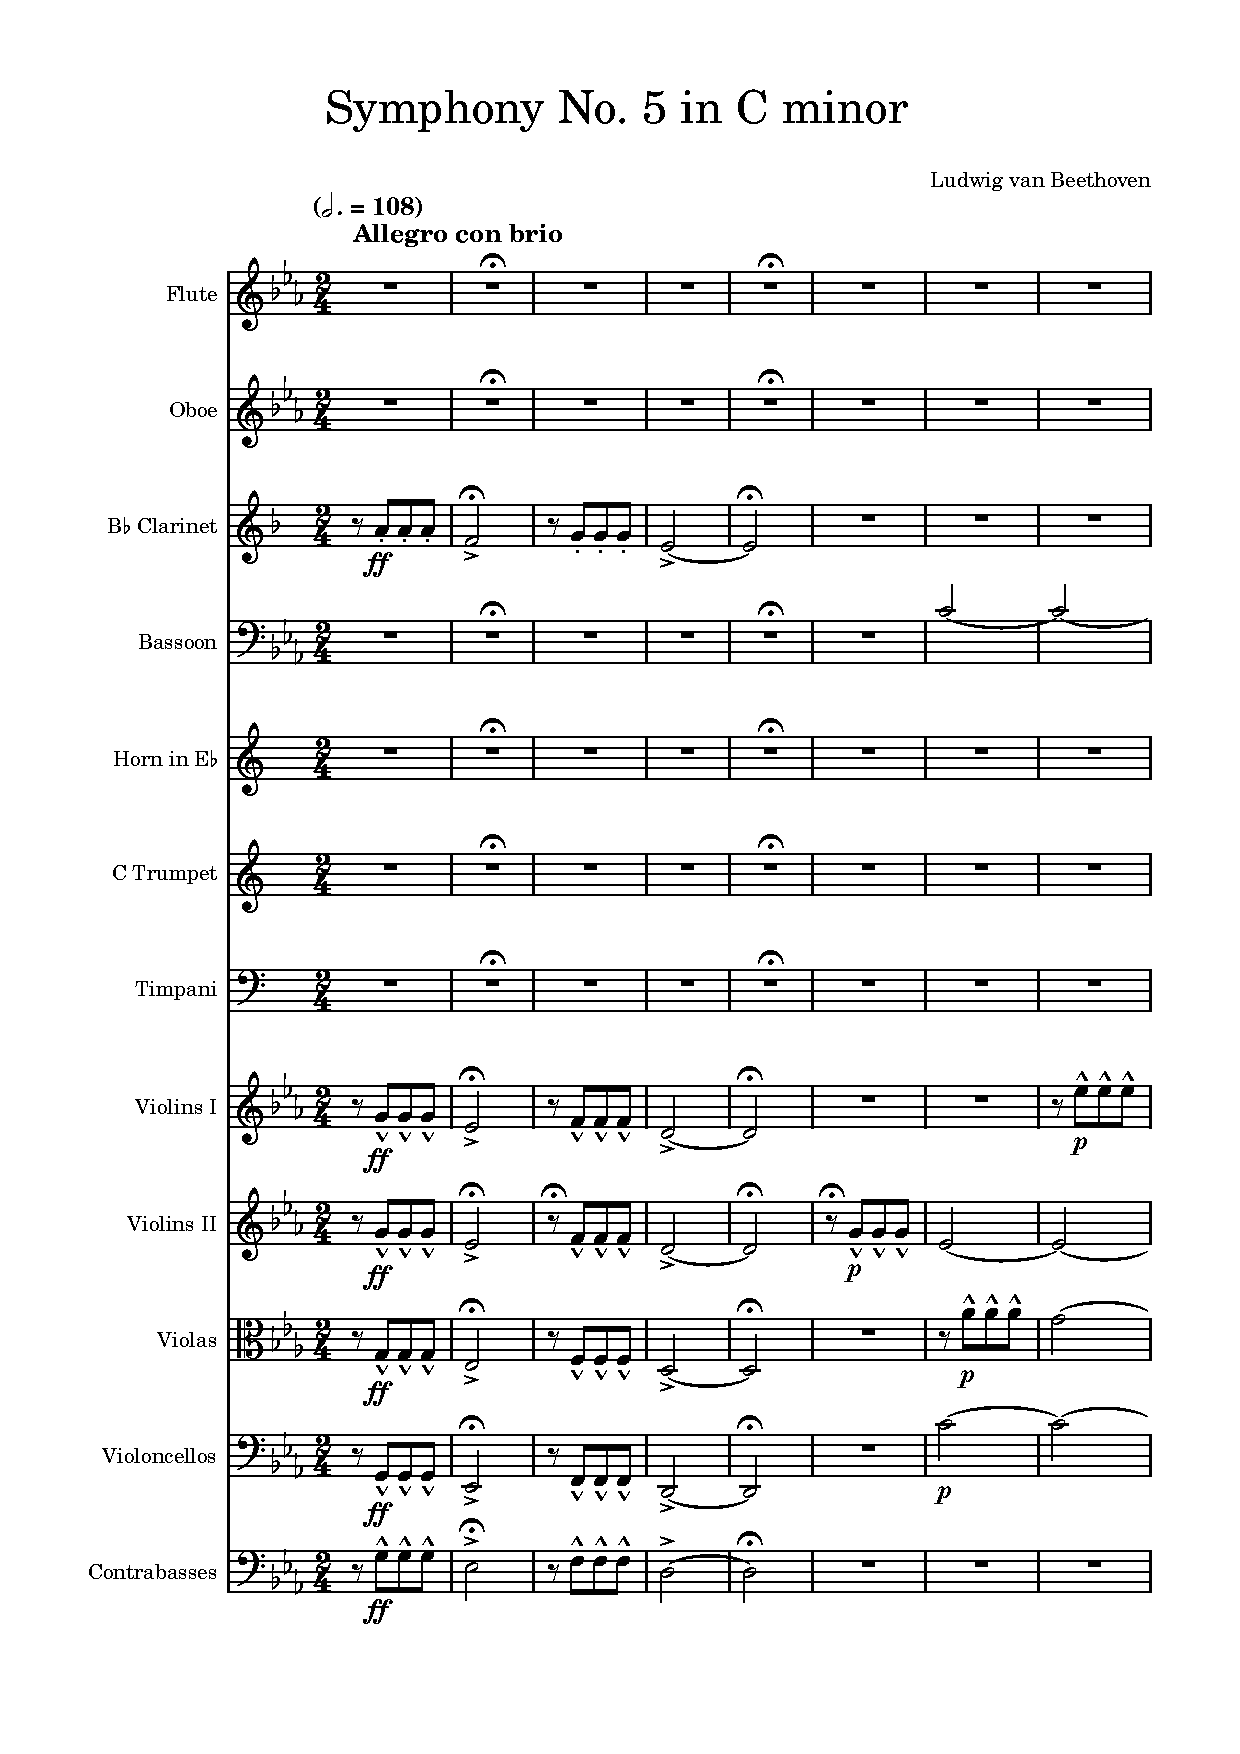
\includegraphics[width=\textwidth,page=1]{beethoven-op67.pdf}
    \caption{Symphony No.\ 5 in C minor, Op.\ 67, by Ludwig van Beethoven, bars 1--8.}
\end{figure}

\section{Test appendix}

Start with an undirected graph $G=(V,E)$ and a set of $n$ colours, which represent the parts for which we are arranging, with each being an independent set. Denote $x_{v,i}$ to be a binary variable such that
\begin{equation*}
    x_{v,i} =
    \begin{cases}
        1 & \text{if vertex $v$ is colour $i$} \\
        0 & \text{otherwise}
    \end{cases}
    \,,
\end{equation*}
which requires $nV$ variables. The energy is
\begin{equation*}
    H = H_A + H_B + H_C + H_D \,.
\end{equation*}

Each vertex is coloured exactly once:
\begin{equation*}
    H_A = A\sum_{v \in V}\left(1-\sum_{i=1}^{n} x_{v,i}\right)^2
\end{equation*}

Vertices of the same colour are not connected by an edge:
\begin{equation*}
    H_B = B\sum_{(u,v) \in E}\sum_{i=1}^n x_{u,i}x_{v,i}
\end{equation*}

Maximise the weighting of selected vertices:
\begin{equation*}
    H_C = -C\sum_{v \in V}\sum_{i=1}^n W_vx_{v,i}
\end{equation*}

Maximise the weighting of included edges:
\begin{equation*}
    H_D = -D\sum_{(u,v)\in E}W_{uv}\sum_{i=1}^n\sum_{j=1}^n x_{u,i}x_{v,j}
\end{equation*}

It can be seen that for $n=1$ this reduces to the MIS problem. For a score with $p$ parts, it will be impossible to colour the graph exactly with $n<p$; the parameter $A$ should be small enough to allow for some vertices to remain uncoloured. The lowest energy solutions will return coloured independent subsets of $G$ that each represents a monophonic part of the final arrangement.

\clearpage

\section*{Scientific summary for a general audience} % 200 words
\addcontentsline{toc}{section}{Scientific summary for a general audience}

The arrangement of music by hand is usually a difficult and time-consuming process, requiring a deep understanding of musical theory and structure. This study aims to automate this process via quantum computing, a technique that relies on the use of qubits, which can exist in a superposition of states. A music score can be split up into a sequence of phrases by looking at how much adjacent notes differ from each other, and turned into a graph representation with nodes and edges, where each node is a phrase, and edges between nodes mean they overlap. This graph can then be sent to a quantum computer in order to select nodes according to a set of rules that determine the properties of the arrangement. Once the nodes have been selected, the corresponding phrases can be reconstructed to create the final score. Here, an excerpt of Beethoven's String Quartet No.\ 10 is reduced to a single part, suitable for a solo instrument.

\end{document}